\chapter{Methodology}

This chapter describes the methodology of the evaluation as well as its application. Running empirical research poses some issues in terms of definition of the hypotheses, replicability of the results and their reporting -- among other factors. To ease the formulation of the goals of the current thesis and to drive the reporting of the results, we decided to use the framework proposed by Victor Basili of the University of Maryland, College Park and the Software Engineering Laboratory at the NASA Goddard Space Flight Center\todo{citation needed} called \textit{Goal Question Metric} (or just GQM).

\section{The Goal Question Metric Approach}

The focus of the GQM approach is to define a good measurement mechanism mainly for engineering disciplines like software engineering, computer science and others. Application of this approach helps support project planning, determine pros and cons of the current project and process, provide an intuition about the impact of modifying or refining a technique as well as assess current progress and last but not least to write the final work in a comprehensible and structured way.

The first prominent step in terms of GQM is to define a set of goals. Goals are entities that are to be assessed and therefore must be defined in a way that allows their assessment. Second step is to define a set of questions, these characterize the way the assessment of a goal is going to be carried out. The last step at the very bottom is to define metrics that are used to answer the questions in a quantitative way. the usual workflow is to define goals and then refine each into several separate questions. The questions are then further refined into metrics where more than one question can have the same metric in common.

\section{Application of GQM}

In this section, we apply the GQM methodology to our project. We proceed from top to bottom (i.e. from goals to metrics) as defined by Basili.

\subsection{Goals}

First, we define goals. In our case, there is only one general goal that looks like this:

\begin{framed}
  \hypertarget{goal:1}{Goal 1:}
  \begin{quote}
    Analyze \textbf{machine learning models} in order to \textbf{find the best possible approach} with respect to \textbf{assignee prediction} from the point of view of \textbf{project managers} in the context of \textbf{issue tracking systems}.
  \end{quote}
\end{framed}

\subsection{Questions}

Next, we need to refine questions for our single goal. We define seven questions, each one addressing a different concern of our research.

\begin{framed}
  \hypertarget{question:1}{Question 1:}
  \begin{quote}
    Is the performance of the model better than performance of the baseline model?
  \end{quote}

  \hypertarget{question:2}{Question 2:}
  \begin{quote}
    How many times does the model predict the correct assignee?
  \end{quote}

  \hypertarget{question:3}{Question 3:}
  \begin{quote}
    How many times does the model predict the correct assignee if the distribution of bug reports is unbalanced?
  \end{quote}

  \hypertarget{question:4}{Question 4:}
  \begin{quote}
    Does the model with the same parameters work with all projects (a projects is a dataset of bug reports)?
  \end{quote}

  \hypertarget{question:5}{Question 5:}
  \begin{quote}
    Is there a difference between open source and proprietary data?
  \end{quote}

  \hypertarget{question:6}{Question 6:}
  \begin{quote}
    Do different time-windowing strategies for training and testing impact the results in terms of performance?
  \end{quote}

  \hypertarget{question:7}{Question 7:}
  \begin{quote}
    How many times is the correct assignee present in a list of more than one top predictions?
  \end{quote}

\end{framed}

\subsection{Metrics}

The last step is to define metrics used to answer questions above. We use five metrics:

\begin{framed}
  \hypertarget{metric:a}{Accuracy:}
  \begin{quote}
    The amount of correctly predicted assignees over all tested predictions, formally:
    $$Accuracy = \frac{tp+tn}{tp+tn+fp+fn}$$
  \end{quote}

  \hypertarget{metric:p}{Macro-Averaged Precision:}
  \begin{quote}
    The amount of assignees correctly predicted as positive for given test sample over number of assignees either correctly or incorrectly predicted as positive, averaged over all classes\cite{Asch2013}, formally:
    $$Precision_{macro} = \frac{1}{q}\sum_{\lambda=1}^q\frac{tp_{\lambda}}{tp_{\lambda}+fp_{\lambda}}$$
  \end{quote}

  \hypertarget{metric:r}{Macro-Averaged Recall:}
  \begin{quote}
    The amount of assignees correctly predicted as positive for given test sample over number of assignees correctly predicted as positive or incorrectly predicted as negative, averaged over all classes\cite{Asch2013}, formally:
    $$Recall_{macro} = \frac{1}{q}\sum_{\lambda=1}^q\frac{tp_{\lambda}}{tp_{\lambda}+fn_{\lambda}}$$ 
  \end{quote}

  \hypertarget{metric:da}{Delta Accuracy:}
  \begin{quote}
    The difference between the accuracy of two models trained and tested on two different datasets:
    $$\Delta Accuracy = |Accuracy^{(X_1)} - Accuracy^{(X_2)}|$$
  \end{quote}

  \hypertarget{metric:dp}{Delta Macro-Averaged Precision:}
  \begin{quote}
    The difference between the macro-averaged precision of two models trained and tested on two different datasets:
    $$\Delta Precision_{macro} = |Precision_{macro}^{(X_1)} - Precision_{macro}^{(X_2)}|$$
  \end{quote}

  \hypertarget{metric:dr}{Delta Macro-Averaged Recall:}
  \begin{quote}
    The difference between the macro-averaged recall of two models trained and tested on two different datasets:
    $$\Delta Recall_{macro} = |Recall_{macro}^{(X_1)} - Recall_{macro}^{(X_2)}|$$
  \end{quote}

  \hypertarget{metric:chi}{Chi-Square Test:}
  \begin{quote}
    Test to assert whether two samples are from the same distribution. The test is performed by calculating the chi-square value and looking up a corresponding value in a chi-square table. The value can be calculated like this ($E$ is expected value and $O$ is observed value):
    $$\chi^2 = \sum\frac{(O - E)^2}{E}$$
  \end{quote}

  \hypertarget{metric:tt}{T-Test:}
  \begin{quote}
    Test to assert whether two samples have the same population mean. The test is performed by first calculating the t-test value and looking up a corresponding value in a t-test table. The value can be calculated like this ($\bar{x}$ is mean, $s^2$ is sample variance and $n$ is number of terms in a set):
    $$t = \frac{\bar{x_1} - \bar{x_2}}{\sqrt{\frac{s_1^2}{n_1} - \frac{s_2^2}{n_2}}}$$
  \end{quote}
\end{framed}

\begin{landscape}
\subsection{Overview}

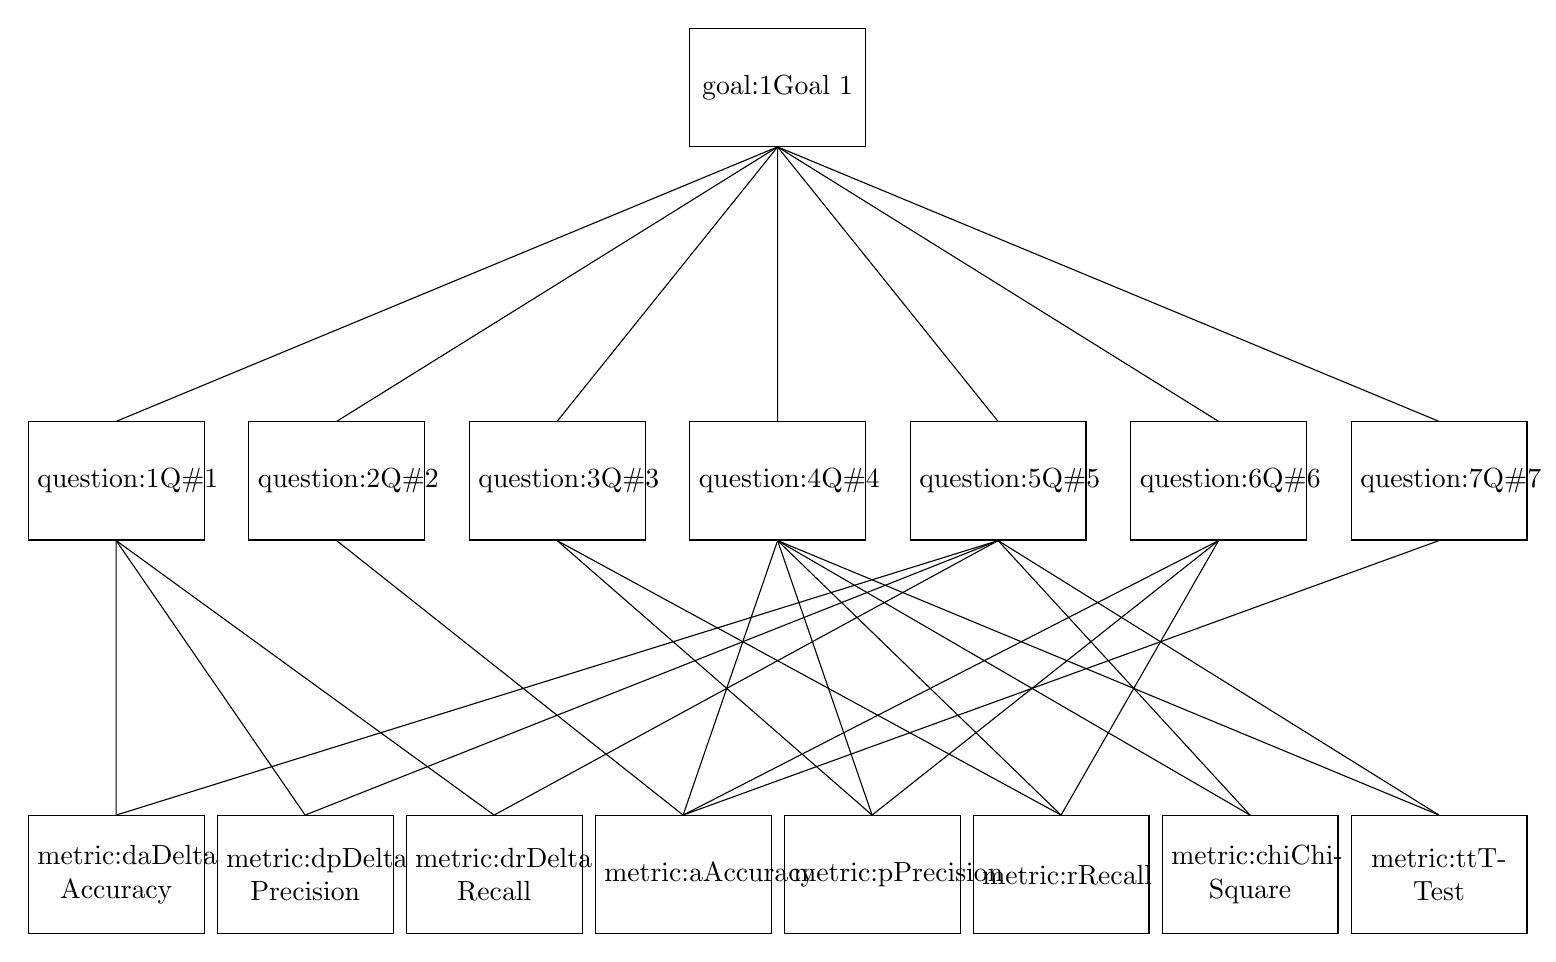
\begin{tikzpicture}
  [auto,every node/.style={rectangle, draw, text centered, text width=2cm,minimum height=1.5cm },node distance=6cm]
\tikzset{
  level 1/.style={sibling distance = 2.8cm, level distance=5cm, edge from parent path={(\tikzparentnode.south) -- (\tikzchildnode.north)}}
}
  \node { \hyperlink{goal:1}{Goal 1} }
    child {node (Q1) { \hyperlink{question:1}{Q\#1} }}
    child {node (Q2) { \hyperlink{question:2}{Q\#2} }}
    child {node (Q3) { \hyperlink{question:3}{Q\#3} }}
    child {node (Q4) { \hyperlink{question:4}{Q\#4} }}
    child {node (Q5) { \hyperlink{question:5}{Q\#5} }}
    child {node (Q6) { \hyperlink{question:6}{Q\#6} }}
    child {node (Q7) { \hyperlink{question:7}{Q\#7} }};

  \node (da) at (-8.4,-10) { \hyperlink{metric:da}{Delta\\Accuracy} };
  \node (dp) at (-6,-10) { \hyperlink{metric:dp}{Delta\\Precision} };
  \node (dr) at (-3.6,-10) { \hyperlink{metric:dr}{Delta\\Recall} };

  \node (a) at (-1.2,-10) { \hyperlink{metric:a}{Accuracy} };
  \node (p) at (1.2,-10) { \hyperlink{metric:p}{Precision} };
  \node (r) at (3.6,-10) { \hyperlink{metric:r}{Recall} };

  \node (chi) at (6,-10) { \hyperlink{metric:chi}{Chi-Square} };
  \node (tt) at (8.4,-10) { \hyperlink{metric:tt}{T-Test} };

  \begin{scope}
    \draw (Q1.south) -- (da.north);
    \draw (Q1.south) -- (dp.north);
    \draw (Q1.south) -- (dr.north);

    \draw (Q2.south) -- (a.north);

    \draw (Q3.south) -- (p.north);
    \draw (Q3.south) -- (r.north);

    \draw (Q4.south) -- (chi.north);
    \draw (Q4.south) -- (tt.north);
    \draw (Q4.south) -- (a.north);
    \draw (Q4.south) -- (p.north);
    \draw (Q4.south) -- (r.north);

    \draw (Q5.south) -- (chi.north);
    \draw (Q5.south) -- (tt.north);
    \draw (Q5.south) -- (da.north);
    \draw (Q5.south) -- (dp.north);
    \draw (Q5.south) -- (dr.north);

    \draw (Q6.south) -- (a.north);
    \draw (Q6.south) -- (p.north);
    \draw (Q6.south) -- (r.north);

    \draw (Q7.south) -- (a.north);
  \end{scope}
\end{tikzpicture}
\end{landscape}